%-----------------------------------------------------------------------------
%
%               Template for sigplanconf LaTeX Class
%
% Name:         sigplanconf-template.tex
%
% Purpose:      A template for sigplanconf.cls, which is a LaTeX 2e class
%               file for SIGPLAN conference proceedings.
%
% Guide:        Refer to "Author's Guide to the ACM SIGPLAN Class,"
%               sigplanconf-guide.pdf
%
% Author:       Paul C. Anagnostopoulos
%               Windfall Software
%               978 371-2316
%               paul@windfall.com
%
% Created:      15 February 2005
%
%-----------------------------------------------------------------------------


\documentclass{sigplanconf}

% The following \documentclass options may be useful:

% preprint      Remove this option only once the paper is in final form.
% 10pt          To set in 10-point type instead of 9-point.
% 11pt          To set in 11-point type instead of 9-point.
% authoryear    To obtain author/year citation style instead of numeric.

\usepackage{amsmath}
\usepackage{listings,xspace}
\usepackage{amsthm}
\usepackage{mdframed}
\usepackage{xcolor}
% \usepackage{fontspec}
\usepackage{graphicx}
\usepackage{setspace}
% \usepackage{booktabs}
\usepackage{wasysym}
\usepackage{amsthm}
\usepackage{url}

\usepackage{caption}
\usepackage{subcaption}

% \usepackage{bcprules}
% \usepackage{prooftree}
\usepackage{multicol}

\lstdefinelanguage{Scala}%
{morekeywords={abstract,case,catch,char,class,%
    def,else,extends,final,%
    if,import,%
    match,module,new,null,object,override,package,private,protected,%
    public,return,super,this,throw,trait,try,type,val,var,with,implicit,%
    macro,sealed,%
  },%
  sensitive,%
  morecomment=[l]//,%
  morecomment=[s]{/*}{*/},%
  morestring=[b]",%
  morestring=[b]',%
  showstringspaces=false%
}[keywords,comments,strings]%

\lstset{language=Scala,%
  mathescape=true,%
  columns=[c]fixed,%
  basewidth={0.5em, 0.40em},%
  basicstyle=\tt,%
  xleftmargin=0.0cm
}

\theoremstyle{definition}
\newmdtheoremenv[hidealllines=true,topline=true,bottomline=true,skipabove=\baselineskip,skipbelow=\baselineskip]{defn}{Definition}[section]

\theoremstyle{definition}
\newmdtheoremenv[hidealllines=true,topline=true,bottomline=true,skipabove=\baselineskip,skipbelow=\baselineskip]{prop}{Property}[section]

% \theoremstyle{nonumberplain}
% \theoremstyle{definition}
% \newmdtheoremenv*[hidealllines=true,topline=true,bottomline=true,skipabove=\baselineskip,skipbelow=\baselineskip]{defnn}{Definition}[section]
\newtheorem*{defn*}{Definition}

% \newtheorem{defn}{Definition}[section]
% \newenvironment{defn}
  % {\begin{mdframed}[style=warning]\begin{mdef}}
  % {\end{mdef}\end{mdframed}}

% comments and notes
\newcommand{\comment}[1]{}
\newcommand{\note}[1]{{\bf $\clubsuit$ #1 $\spadesuit$}}
\newcommand{\ifreport}[1]{#1}
%\newcommand{\ifreport}[1]{}

\newcommand{\todo}{{\bf \colorbox{red}{\color{white}TODO:}}}
\newcommand{\ie}{{\em i.e.,~}}
\newcommand{\eg}{{\em e.g.,~}}
\newcommand{\term}[1]{\mbox{\texttt{#1}}}
\newcommand{\itl}[1]{\mbox{\textit{#1}}}

% commas and semicolons
\newcommand{\comma}{,\,}
\newcommand{\commadots}{\comma \ldots \comma}
\newcommand{\semi}{;\mbox{;};}
\newcommand{\semidots}{\semi \ldots \semi}

% spacing
\newcommand{\gap}{\quad\quad}
\newcommand{\biggap}{\quad\quad\quad}
\newcommand{\nextline}{\\ \\}
\newcommand{\htabwidth}{0.5cm}
\newcommand{\tabwidth}{1cm}
\newcommand{\htab}{\hspace{\htabwidth}}
\newcommand{\tab}{\hspace{\tabwidth}}
\newcommand{\linesep}{\ \hrulefill \ \smallskip}

\newcommand{\sectionline}{%
  \nointerlineskip \vspace{\baselineskip}%
  \hspace{\fill}\rule{0.5\linewidth}{.7pt}\hspace{\fill}%
  \par\nointerlineskip \vspace{\baselineskip}
}

% figures
\newcommand{\figurebox}[1]
        {\fbox{\begin{minipage}{\textwidth} #1 \medskip\end{minipage}}}
\newcommand{\twofig}[3]
        {\begin{figure*}[t]#3\ \hrulefill\
        \caption{\label{#1}#2}\end{figure*}}
\newcommand{\boxfig}[3]
        {\begin{figure*}\figurebox{#3\caption{\label{#1}#2}}\end{figure*}}
\newcommand{\figref}[1]
        {Figure~\ref{#1}}

% arrays
\newcommand{\ba}{\begin{array}}
\newcommand{\ea}{\end{array}}
\newcommand{\bda}{\[\ba}
\newcommand{\eda}{\ea\]}
\newcommand{\ei}{\end{array}}
\newcommand{\bcases}{\left\{\begin{array}{ll}}
\newcommand{\ecases}{\end{array}\right.}

%%%%%%%%%%%%%%%%%%%%%%%%%%%%%%%%%%%%%%%
%   Language abstraction commands     %
%%%%%%%%%%%%%%%%%%%%%%%%%%%%%%%%%%%%%%%

%% Relations
% Subtype
\newcommand{\sub}{<:}
% Type assignment
\newcommand{\typ}{:}
% reduction
\newcommand{\reduces}{\;\rightarrow\;}
% well-formedness
\newcommand{\wf}{\;\mbox{\textbf{wf}}}

%% Operators
% Type selection
\newcommand{\tsel}{\#}
% Function type
\newcommand{\tfun}{\rightarrow}
\newcommand{\dfun}[3]{(#1\!:\!#2) \Rightarrow #3}
% Conjunction
\newcommand{\tand}{\wedge}
% Disjunction
\newcommand{\tor}{\vee}
% Singleton type suffix
\newcommand{\sing}{.\textbf{type}}

%% Syntax
% Header for typing rules
\newcommand{\judgement}[2]{{\bf #1} \hfill \fbox{#2}}
% Refinement
\newcommand{\refine}[2]{\left\{#1 \Rightarrow #2 \right\}}
% Field definitions
\newcommand{\ldefs}[1]{\left\{#1\right\}}
% Member sequences
\newcommand{\seq}[1]{\overline{#1}}
% Lambda
\newcommand{\dabs}[3]{(#1\!:\!#2)\Rightarrow #3}
\newcommand{\abs}[3]{\lambda #1\!:\!#2.#3}
% Application
\newcommand{\app}[2]{#1\;#2}
% Substitution
\newcommand{\subst}[3]{[#1/#2]#3}
% Object creation
\newcommand{\new}[3]{\textbf{val }#1 = \textbf{new }#2 ;\; #3}
%\renewcommand{\new}[3]{#1 \leftarrow #2 \,\textbf{in}\, #3}
% Field declaration
\newcommand{\Ldecl}[3]{#1 \typ #2..#3}%{#1 \operatorname{>:} #2 \operatorname{<:} #3}
\newcommand{\ldecl}[2]{#1 \typ #2}
% Top and Bottom
\newcommand{\Top}{\top}%{\textbf{Top}}
\newcommand{\Bot}{\bot}%\textbf{Bot}}
% Environment extension
\newcommand{\envplus}[1]{\uplus \{ #1 \}}

\newcommand{\reduction}[4]{#1, #2 \reduces #3, #4}
\newcommand{\reducebig}[6]{#1, #2, #3 \;\Downarrow\; #4, #5, #6}
\newcommand{\evaluate}[5]{#1, #2, #3 \;\Downarrow\; #4, #5}
\newcommand{\evalcap}[8]{#1, #2, #3, #4 \;\Downarrow\; #5, #6, #7, #8}
\newcommand{\evalcapbreak}[8]{#1, #2, #3, #4 \;\Downarrow\; \\ #5, #6, #7, #8}
\newcommand{\evalcapfin}[9]{#2, #3, #4, #5 \;\Downarrow_{#1}\; #6, #7, #8, #9}

\newcommand{\sframe}[3]{\langle #1, #2, #3 \rangle}
\newcommand{\stack}[4]{#1 \sframe {#2} {#3} {#4}}
\newcommand{\reduce}[4]{#1, #2 \;\longrightarrow\; #3, #4}
\newcommand{\reducebreak}[4]{#1, #2 \\ \;\longrightarrow\; #3, #4}

\newcommand{\sreduce}[6]{#1, #2, #3 \;\longrightarrow\; #4, #5, #6}
\newcommand{\sreducebreak}[6]{#1, #2, #3 \\ \;\longrightarrow\; #4, #5, #6}
\newcommand{\sreducestar}[6]{#1, #2, #3 \;\longrightarrow^{\ast}\; #4, #5, #6}
\newcommand{\sreducestarbreak}[6]{#1, #2, #3 \\ \;\longrightarrow^{\ast}\; #4, #5, #6}

% misc identifiers
\newcommand{\dom}{\mbox{\sl dom}}
\newcommand{\fn}{\mbox{\sl fn}}
\newcommand{\bn}{\mbox{\sl bn}}
\newcommand{\sig}{\mbox{\sl sig}}
\newcommand{\IF}{\mbox{\mathem if}}
\newcommand{\OTHERWISE}{\mbox{\mathem otherwise}}
\newcommand{\strongexpand}{\prec\!\!\prec}
\newcommand{\weakexpand}{\prec}
\newcommand{\spcomma}{~,~}

\makeatletter
\def\@copyrightspace{\relax}
\makeatother


\begin{document}

\special{papersize=8.5in,11in}
\setlength{\pdfpageheight}{\paperheight}
\setlength{\pdfpagewidth}{\paperwidth}

% \conferenceinfo{CONF 'yy}{Month d--d, 20yy, City, ST, Country}
% \copyrightyear{20yy}
% \copyrightdata{978-1-nnnn-nnnn-n/yy/mm}
% \doi{nnnnnnn.nnnnnnn}

% Uncomment one of the following two, if you are not going for the
% traditional copyright transfer agreement.

%\exclusivelicense                % ACM gets exclusive license to publish,
                                  % you retain copyright

%\permissiontopublish             % ACM gets nonexclusive license to publish
                                  % (paid open-access papers,
                                  % short abstracts)

% \titlebanner{banner above paper title}        % These are ignored unless
% \preprintfooter{short description of paper}   % 'preprint' option specified.

\title{Function-Passing Style: Typed, Distributed Functional Programming}
% \subtitle{Subtitle Text, if any}

\authorinfo{Heather Miller}
           {EPFL}
           {heather.miller@epfl.ch}
\authorinfo{Philipp Haller}
           {KTH Royal Institute of Technology}
           {phaller@kth.se}

\maketitle

\begin{abstract}
This is the text of the abstract.
\end{abstract}

% \category{CR-number}{subcategory}{third-level}

% general terms are not compulsory anymore,
% you may leave them out
% \terms
% term1, term2

% \keywords
% keyword1, keyword2

\section{Introduction}

From the ivory tower, it may not be evident,
% It might not seem this way from the ivory tower,
but mainstream software development has become largely distributed. Two trends
dominate the current landscape; systems composed of (1) microservices,
 % or designed to be software as a service (SaaS),
and (2) systems for ``big data''
processing.

Yet, software developers still fumble with low-level RPC frameworks.
% and sluggish serialization frameworks.
Mainstream programming languages have traditionally offered little support in
this space.

In mainstream software development, there are two trends on the rise.
Data-centric systems, and systems for ``big data'' on the rise. As a matter of fact, services and systems that are simply ``connected'' to others are on the rise. The trend is called ``microservices'' and a piece of software that a user might perceive as a single piece of software might be made up of dozens of such microservices--complex applications are composed of small, independent processes communicating with each other using language-agnostic APIs.
This is the landscape of modern software development.
These are all distributed applications.
programming languages remain firmly rooted in a single-machine design. Developers of services and systems pushing the envelope today are distributed; they must either synchronize with.

We design module systems, etc, for maximum reuse and productivity, we go as
far as we can to demonstrate their power. But we often . Some of these
concerns have been affectionately referred to as the ``awkward
squad''~\cite{AwkwardSquad} by PL research, and they are concerns that are central to
contemporary software development.

Functional programming brings value to distributed systems builders. The
success of popular Spark can be attributed to functional ideas.

However, beyond Spark's interface, .

We refer to the model as {\em function-passing}, and .










We design a programming model in such a way that we can ``maximize'' static
types, and with it enable type-specialized picklers (statically generated),
typed closures, and type-specialized data structures.

The motto is ``making type inference work for you when optimizing distributed
systems'', or ``how type inference and existential types benefit distributed
systems''.

In existing systems, types are only in the user-facing API and help the user.
However, all too often, the internals of a distributed system are largely
untyped, in particular when operating on data types that are also shipped
remotely. In our approach we now go ahead and make types work so that they
benefit both users (helping catch common errors) \emph{and} distributed
systems builders. Our approach leverages types to provide (1) type-specialized
picklers, and (2) type-specialized collections/builders.

The approach is novel, because noone talks about making sure the unpicklers
and builders themselves are serializable, but that's actually fundamental to
the whole design.

\begin{itemize}

\item We have to make the point that serialization is like a primitive in
systems design, not some extra thing you figure out how to do later, like in
typical PLs. so maybe one central point that we should try to make is that
for distributed systems, serializability is like a key primitive, along with
latency and other things.

\item we want to prove that typed distributed systems are a good idea. right
now a lot of systems for dist computing are fundamentally untyped or
dynamically checked. those that are typed lose type information between
machines.

\item so we're trying to argue that types are good for system builders.

\end{itemize}

The fact that actually these benefits from types \emph{carry over to other
models as well} (not just spark-like models).


Generalization of MapReduce model. Low-level. Inversion of the actor model.
Can represent different many models for distributed computing, e.g. Spark,
Percolator (we probably can't validate this claim.)

Illustrations to have:
\begin{enumerate}
\item nice figure
\item organic evolving model on youtube
\end{enumerate}

\subsection{Model}

This is the basic model.

\begin{figure}[ht!]
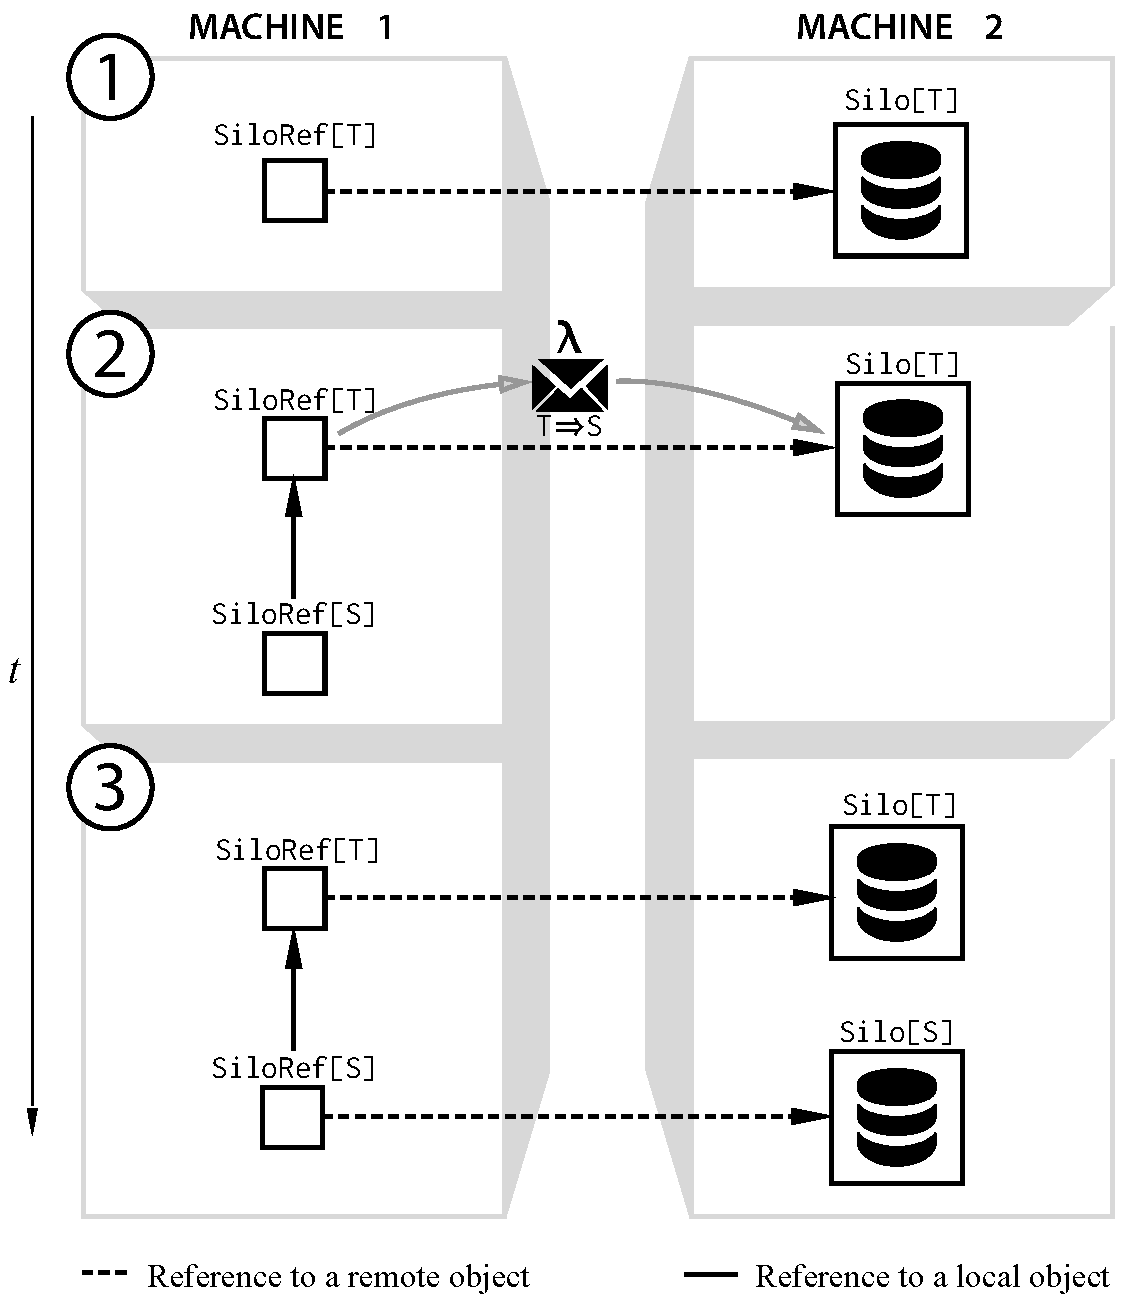
\includegraphics[width=\columnwidth]{basic-diagram.pdf}
\caption{Basic model.}\label{fig:basic-diagram}
\end{figure}


Nothing beats a video when something evolves in space in time, so we've also produced a short video to illustrate the model\footnote{\url{https://vimeo.com/120415626}}

\subsection{Evaluation}

we could make the performance eval strong by saying, ok, we implemented real
apps, so we have the real communication that needs to happen (and happens).
and we now make this communication typed, plus we measure exactly the
percentage of time that's spent in serialization for example. and then we
could even interpolate the results, so we could say, ok, if some other dist
system has a lower percentage spent in serialization, then the speed up would
be like this.

and then we could even measure that for real spark, and then interpolate and
say, ok, in the ideal case, meaning using all of our design principles, we
could speed up things like this, if one would re-architect spark to preserve
types (it's a huge task, so out of scope).

well, it would definitely be something that we can measure objectively. the
only thing we have to guard against would be to say, adding picklers and
builders does not otherwise \emph{degrade} performance, like, we'd have to
prove that there's no cost, but \emph{just} the performance benefits. adding
the classname of the unpickler adds a few bytes to each pickle, for example.

we could even show that with babyspark, like have a version that uses java
serialization, then a version that uses pickling without selfdescribing, then
with runtime unpickling, and with all static. because we have those numbers
for babyspark then the interpolation will be much more precise.



\section{Future Work}

Adapt this model for streaming computation. This would take coming up with a
solution to null out references in the {\em lineage}. This would make it possible to instantiate and populate new silos to handle incoming data.

% \appendix
% \section{Appendix Title}

% This is the text of the appendix, if you need one.

% \acks

% Acknowledgments, if needed.

% We recommend abbrvnat bibliography style.

\bibliographystyle{abbrvnat}

% The bibliography should be embedded for final submission.
\bibliography{bib}

% \begin{thebibliography}{}
% \softraggedright

% \bibitem[Smith et~al.(2009)Smith, Jones]{smith02}
% P. Q. Smith, and X. Y. Jones. ...reference text...

% \end{thebibliography}


\end{document}

%                       Revision History
%                       -------- -------
%  Date         Person  Ver.    Change
%  ----         ------  ----    ------

%  2013.06.29   TU      0.1--4  comments on permission/copyright notices

